\documentclass[11pt,a4paper]{article}
\usepackage[margin=23mm,headheight=14pt,headsep=8.5mm,footskip=10mm]{geometry}
\usepackage{amsmath,amssymb,amsthm}
\usepackage[no-math]{fontspec}
\usepackage{xeCJK}
\setmainfont{Latin Modern Roman}
\setCJKmainfont{FandolSong-Regular.otf}[Script=CustomDefault,Path=assets/fonts/fandol/,BoldFont=FandolSong-Bold.otf,ItalicFont=FandolSong-Regular.otf,BoldItalicFont=FandolSong-Bold.otf]
\setCJKsansfont{FandolSong-Regular.otf}[Script=CustomDefault,Path=assets/fonts/fandol/,BoldFont=FandolSong-Bold.otf]
\xeCJKsetup{PunctStyle=quanjiao,CheckSingle=true}
\usepackage{setspace}
\setstretch{1.12}
\setlength{\parindent}{2em}
\setlength{\parskip}{3pt}
\usepackage{titlesec}
\titleformat{\section}{\centering\normalfont\Large\bfseries}{\thesection.}{0.6em}{}
\titleformat{\subsection}{\normalfont\large\bfseries}{}{0pt}{}
\titlespacing*{\section}{0pt}{1.8\baselineskip}{1.0\baselineskip}
\titlespacing*{\subsection}{0pt}{1.1\baselineskip}{0.5\baselineskip}
\usepackage{enumitem}
\setlist[enumerate]{leftmargin=2em,labelsep=0.5em,itemsep=3pt,parsep=0pt,topsep=6pt}
\providecommand{\tightlist}{\setlength{\itemsep}{3pt}\setlength{\parskip}{0pt}}
\usepackage{needspace}
\newenvironment{statementblock}{\par\Needspace{9\baselineskip}\noindent}{\par\nopagebreak[4]}
\newenvironment{proofblock}{\par\Needspace{4\baselineskip}\noindent}{\par}
\usepackage{fancyhdr}
\pagestyle{fancy}
\fancyhf{}
\fancyhead[L]{\small 数学手记}
\fancyhead[R]{\small 复变函数 · 第六章}
\fancyfoot[C]{\thepage}
\renewcommand{\headrulewidth}{0.4pt}
\usepackage[hidelinks,unicode,bookmarksnumbered=true,linktoc=all]{hyperref}
\usepackage{bookmark}
\bookmarksetup{depth=2}
\hypersetup{pdftitle={复变函数讲义：第六章},pdfauthor={Vincent Arqain},pdfsubject={全纯开拓}}
\renewcommand{\contentsname}{目录}
\setcounter{tocdepth}{1}
\setcounter{secnumdepth}{1}
\widowpenalty=10000
\clubpenalty=10000
\displaywidowpenalty=10000
\predisplaypenalty=10000
\interdisplaylinepenalty=10000
\raggedbottom

\usepackage{tabularx,booktabs,array}
\renewcommand{\thesection}{6.\arabic{section}}
\emergencystretch=2em

\usepackage{graphicx}
\usepackage{longtable}
\usepackage{calc}
\usepackage{float}
\floatplacement{figure}{H}
\renewcommand{\figurename}{图}
\makeatletter
\def\maxwidth{\ifdim\Gin@nat@width>\linewidth\linewidth\else\Gin@nat@width\fi}
\def\maxheight{\ifdim\Gin@nat@height>0.72\textheight0.72\textheight\else\Gin@nat@height\fi}
\makeatother
\setkeys{Gin}{width=\maxwidth,height=\maxheight,keepaspectratio}
\providecommand{\pandocbounded}[1]{#1}
\setcounter{tocdepth}{2}
\begin{document}
\begin{center}
{\LARGE\bfseries 复变函数讲义\par}
\vspace{8pt}{\large 第六章\quad 全纯开拓\par}
\vspace{6pt}{\small 依史济怀、刘太顺《复变函数》\quad 教材第 194—209 页\par}
\end{center}\vspace{8pt}
本章含3节讲义及全部 28 道习题原题。定义、定理和性质沿用教材的记号与编号；证明补足必要条件、退化情形与关键推导。覆盖 19 个教材编号条目，补足可求长曲线的连续拼接、单叶反射的同侧条件、圆环分类及路径同伦证明。Picard 小定理复用已证的导数估计，使证明依赖在前六章内闭合；保留九幅教材配图、逐节索引与原题校注。习题不附解答，原题中的疑义另列校勘。
\begingroup\setlength{\parskip}{0pt}\tableofcontents\endgroup\clearpage
\section{Schwarz 对称原理}
对应教材第 194---201
页。全纯开拓的目标是扩大函数的定义域，同时在原域保持原值。若
\(G\subset D\) 都是域，\(f\in H(G)\)，\(F\in H(D)\) 且 \(F|_G=f\)，就称
\(F\) 为 \(f\) 到 \(D\)
的全纯开拓。同一连通目标域上的开拓若存在，由唯一性定理必唯一；这句话并不排除沿不同路径到达同一点时出现不同函数元。

\Needspace{8\baselineskip}
\subsection{定理 6.1.1：Painlevé 连续开拓原理}\label{ch06-s1-heading-1}

设 \(D\) 是域，\(\gamma_1,\ldots,\gamma_m\) 为有限条可求长曲线。若
\(f\in C(D)\) 且在 \(D\setminus\bigcup_{j=1}^m\gamma_j\) 上全纯，则
\(f\in H(D)\)。

证明：取闭正方形 \(Q\Subset D\)，把它分成边长 \(h\)
的小正方形。设曲线总长度为 \(L\)。每条曲线按弧长分成长度不超过 \(h\)
的小段；每段包含于以其起点为中心、半径 \(h\)
的圆盘。这样的圆盘至多碰到固定数目的网格方格，故碰到曲线的小方格数满足

\[
N(h)\le C(L/h+m).\qquad\text{(6.1.1)}
\]

未碰到曲线的小方格上，Cauchy
定理给出边界积分为零。若仅在边界接触曲线，也将其归入碰到曲线的方格。在这样的方格
\(Q_\nu\) 中任选 \(z_\nu\)，利用常数的闭路积分为零，得到

\[
\left|\int_{\partial Q_\nu}f(z)\,dz\right|
=\left|\int_{\partial Q_\nu}[f(z)-f(z_\nu)]\,dz\right|
\le 4h\,\omega(\sqrt2h),\qquad\text{(6.1.2)}
\]

其中 \(\omega\) 是 \(f\) 在 \(Q\)
上的一致连续模。所有小方格相加，内部边抵消，因此

\[
\left|\int_{\partial Q}f(z)\,dz\right|
\le4C(L+mh)\omega(\sqrt2h)\longrightarrow0.
\]

对轴平行矩形作边长可比的网格划分，同样得到一切内含矩形的边界积分为零。局部沿先水平、后竖直的折线积分定义原函数，矩形积分为零保证交换两段次序不改变结果。连续性说明该原函数的偏导分别为
\(f\) 和 \(if\)，故其微分为 \(f(z)\,dz\)，它全纯且导数为
\(f\)；由全纯函数导数全纯，得 \(f\in H(D)\)。这也证明了所用的矩形版
Morera 判据。

``曲线可求长''用于控制坏方格总边长，``函数连续''使每格振幅趋于零。一般曲线可能与边界相交无穷多次，不能直接把积分口头拆成有限个简单区域。

\Needspace{8\baselineskip}
\subsection{定理 6.1.2：实轴反射}\label{ch06-s1-heading-2}

设域 \(D\) 关于实轴对称，记 \(D^+=D\cap\{\operatorname{Im}z>0\}\)。若
\(f\) 在 \(D^+\) 全纯，在 \(D^+\cup(D\cap\mathbb R)\) 连续，且在
\(D\cap\mathbb R\) 上取实值，则

\[
F(z)=\begin{cases}
f(z),&\operatorname{Im}z\ge0,\\
\overline{f(\bar z)},&\operatorname{Im}z<0
\end{cases}\qquad\text{(6.1.3)}
\]

给出 \(D\) 上唯一的全纯开拓，并满足 \(F(\bar z)=\overline{F(z)}\)。

证明：若 \(f(w)=\sum a_n(w-w_0)^n\)，则反射一侧的表达式为
\(\sum\bar a_n(z-\bar w_0)^n\)，所以在那里全纯。实轴上的实值条件恰使两侧极限一致。对实轴每点取小圆盘，以其中的有限线段应用定理
6.1.1，便知拼接后全纯。对称恒等式由定义得到，唯一性由内部唯一性定理得到。

更一般地，若边界值在直线 \(w_0+e^{i\theta}\mathbb R\) 上，先对函数作
\(e^{-i\theta}(f-w_0)\)，反射后再变回。对该直线的反射为
\(w\mapsto w_0+e^{2i\theta}\overline{w-w_0}\)。若源直线不是实轴，先作相应平移、旋转，证明完全相同。

\Needspace{8\baselineskip}
\subsection{定理 6.1.3：圆周反射与亚纯版本}\label{ch06-s1-heading-3}

对圆周 \(\gamma=\{|z-a|=r\}\)、\(\Gamma=\{|w-b|=\rho\}\)，记反射

\[
\sigma_\gamma(z)=a+\frac{r^2}{\overline{z-a}},\qquad
\sigma_\Gamma(w)=b+\frac{\rho^2}{\overline{w-b}}.
\qquad\text{(6.1.4)}
\]

在球面上约定
\(\sigma_\gamma(a)=\infty\)、\(\sigma_\gamma(\infty)=a\)。两者均为反全纯对合，固定相应圆周，并交换两侧。

设 \(D\) 关于 \(\gamma\) 对称，\(D^+\) 为其一侧部分。若 \(f\) 在 \(D^+\)
全纯，连续至 \(D\cap\gamma\)，将这段边界映入 \(\Gamma\)，并且 \(f\ne b\)
于 \(D^+\)，则在另一侧定义

\[
F=\sigma_\Gamma\circ f\circ\sigma_\gamma
=b+\frac{\rho^2}{\overline{f(\sigma_\gamma(z))-b}},
\qquad\text{(6.1.5)}
\]

与原来的 \(f\) 拼成全纯开拓。若不要求 \(f\ne b\)，得到的是亚纯开拓；原侧
\(f-b\) 的零点反射为另一侧的极点，阶数相同。

证明：两次反全纯复合使式（6.1.5）在非极点处全纯。边界点 \(\zeta\) 固定于
\(\sigma_\gamma\)，而 \(f(\zeta)\) 固定于
\(\sigma_\Gamma\)，故边界连续性成立。每个圆周点附近是一段可求长弧，应用定理
6.1.1。分母不为零保证没有极点；若 \(f-b\) 有 \(m\)
阶零点，局部代入反射公式得到恰好 \(m\) 阶极点。涉及源点 \(\infty\)
时用坐标 \(1/z\) 作同一证明。若目标允许取
\(\infty\)，应称球面值全纯映射，也就是通常的亚纯函数，不能误称为有限值全纯函数。

圆周、直线混合的反射同样由各自的反射公式复合得到。边界取值在目标圆上是两侧能拼接的条件，省略目标圆心则是有限值开拓没有极点的条件。

\Needspace{8\baselineskip}
\subsection{定理 6.1.4：单叶反射的条件修订}\label{ch06-s1-heading-4}

\textbf{可直接使用的版本。} 在定理 6.1.3 的条件下，另设 \(f\) 在
\(D^+\cup(D\cap\gamma)\) 上单射，且 \(f(D^+)\) 全部位于目标圆 \(\Gamma\)
的同一开侧，则反射开拓 \(F\) 在整个 \(D\) 上单射，因而双全纯地映到
\(F(D)\)。

证明：原侧的单射性已知；反射侧的单射性由两个反射均为一一映射得到。两侧的像位于
\(\Gamma\) 的相反开侧，故不能重合；边界像在 \(\Gamma\)
上，既不与内点像重合，边界点之间也不重合。所以 \(F\)
单射。单射全纯函数的导数不为零，局部反函数拼接成全纯逆映射。

\textbf{原述为什么需要补条件。} 上传教材第 197
页只列单叶性、边界单射、边界落在目标圆和省略圆心，未列出同侧条件。在其允许的直线版本中，取

\[
D=\{z:|\operatorname{Re}z|<1,\ |\operatorname{Im}z|<3\pi/2\},
\qquad f(z)=e^z\quad(z\in D^+).
\]

\(f\) 在上半部连同实轴上单射：两点指数相同只可能相差
\(2k\pi i\)，这里虚部差严格小于 \(3\pi/2\)。实轴像为正实数。但反射后的
\(F=e^z\) 满足 \(F(i\pi)=F(-i\pi)=-1\)，因此不单叶。

这不是仅在直线情形才出现的问题。令
\(S(z)=(z-10i)/(z+10i)\)、\(T(w)=(w-10i)/(w+10i)\)，把上述域变为
\(S(D)\)，函数变为 \(T\circ e^z\circ S^{-1}\)。\(S,T\)
把实轴变为单位圆并保持反射关系；因
\(|e^z|<e<10\)，变换后的函数既无极点又不取目标圆心
\(0\)。它满足教材圆周版的四项条件，但仍在 \(S(i\pi)\) 与 \(S(-i\pi)\)
取同值。这里只把补充条件后的命题标为已证明；另一版本教材的原文或作者修订意图仍未核实。

\Needspace{8\baselineskip}
\subsection{例 6.1.5：周期裂缝上半平面}\label{ch06-s1-heading-5}

设 \(a>0\)，从上半平面删去竖直线段

\[
L_k=\{k\pi+\pi/2+iy:0\le y\le a\},\qquad k\in\mathbb Z,
\]

所得域记为 \(D\)。下图保留教材的裂缝位置与高度。

\noindent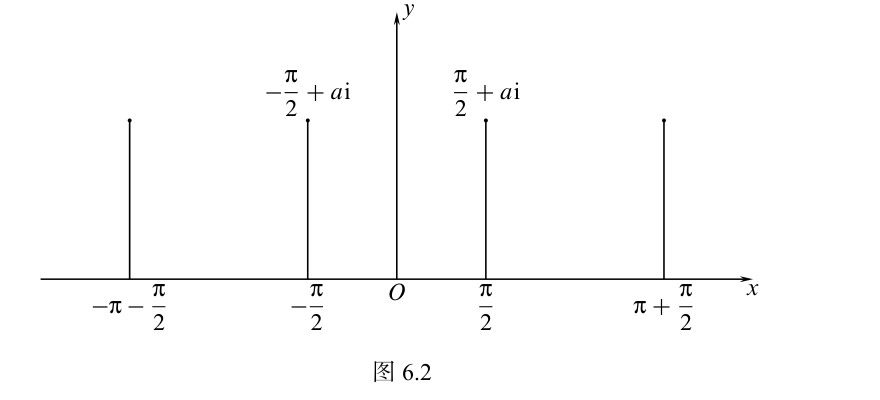
\includegraphics{public/figures/complex-functions/ch06-fig-6-2.png}

令
\(G=\{z:-\pi/2<\operatorname{Re}z<\pi/2,\operatorname{Im}z>0\}\)。先证明
\(\sin:G\to\mathbb C^+\) 双全纯。对
\(z=x+iy\)，\(\operatorname{Im}\sin z=\cos x\sinh y>0\)。又
\(\sin z=\sin w\) 只能有 \(z-w=2k\pi\) 或 \(z+w=(2k+1)\pi\)；在 \(G\)
内前者只给 \(z=w\)，后者因虚部为正不可能。要证满射，注意 \(G\)
的有限边界映入实轴，而 \(y\to\infty\) 时

\[
|\sin(x+iy)|^2=\sin^2x+\sinh^2y\longrightarrow\infty.
\]

于是 \(\sin:G\to\mathbb C^+\)
是适当映射：目标紧集的原像不可能逼近边界或无穷远。它的像既开又闭，且非空，上半平面连通，所以像就是上半平面。局部反函数存在并拼接为全纯逆，记为
\(A:\mathbb C^+\to G\)。因此

\[
h(z)=A\left(\frac{\sin z}{\cosh a}\right)\qquad\text{(6.1.6)}
\]

把 \(G\) 双全纯映为自身。这里 \(A\)
是刚刚确定的逆分支，不能随意代入一个未指定的多值 \(\arcsin\)。在右侧边上
\(\sin(\pi/2+iy)=\cosh y\)；当 \(y>a\) 时，局部逆函数说明 \(h\)
连续延伸并将该开射线映为 \(\pi/2+i(0,\infty)\)，左侧同理。

沿这两条开射线反射，再逐条向左右反射。每次原像、像都在反射直线的一侧，符合修订的定理
6.1.4。所得映射把每条半带
\(G_k=\{k\pi-\pi/2<\operatorname{Re}z<k\pi+\pi/2,\operatorname{Im}z>0\}\)
双全纯映到同一编号的目标半带；两带间保留的射线 \(y>a\)
则映到完整目标分界射线
\(y>0\)。这些开半带及分界射线恰好铺满上半平面，所以得到
\(D\to\mathbb C^+\)
的双全纯映射。任意紧集只遇到有限条分界线，因此这里的无穷次反射没有局部收敛问题。

\Needspace{8\baselineskip}
\subsection{例 6.1.6：圆环的模与全部双全纯映射}\label{ch06-s1-heading-6}

设 \(0<r_1<r_2<\infty\)、\(0<R_1<R_2<\infty\)。圆环
\(A=\{r_1<|z|<r_2\}\) 与 \(B=\{R_1<|w|<R_2\}\) 双全纯等价，当且仅当

\[
\frac{r_2}{r_1}=\frac{R_2}{R_1}.\qquad\text{(6.1.7)}
\]

此时全部映射为

\[
f(z)=e^{i\theta}\frac{R_2}{r_2}z
\quad\text{或}\quad f(z)=e^{i\theta}\frac{r_1R_2}{z},
\qquad\theta\in\mathbb R.\qquad\text{(6.1.8)}
\]

教材通过圆周反射证明，但预先引用了第七章的边界对应。下面直接控制边界模值，补齐本章内的证明。

证明：设 \(f:A\to B\) 双全纯。它是同胚，故目标紧集的逆像紧。给定足够小的
\(\varepsilon>0\)，目标中间闭环
\(R_1+\varepsilon\le|w|\le R_2-\varepsilon\)
的原像离源边界有正距离。因此源圆环的每个足够窄的边界领圈，都被映入目标的两个边界领圈之一；源领圈连通，不能同时进入两者。随着领圈缩小，其选择不变，因为不同边界的领圈不相交。两个源边界必须对应两个不同目标边界：若都对应同一边界，取趋向另一目标边界的点及其原像，原像在源闭环中的聚点既不可能在内部，也不可能在任何边界，矛盾。

先设对应次序不交换。上述论证说明 \(\log|f(z)|\)
连续延伸到两条边界，边值分别为 \(\log R_1\)、\(\log R_2\)。定义

\[
\alpha=\frac{\log(R_2/R_1)}{\log(r_2/r_1)},\qquad
\beta=\log R_1-\alpha\log r_1.
\]

\(u=\log|f|-\alpha\log|z|-\beta\)
局部为全纯函数的实部，且边值全零。这样的实部满足最大、最小原理：局部取全纯函数
\(g\)，对 \(e^g\)
用最大模原理即可；若内部取得极值，局部常值，再由连通性传播。因此
\(u=0\)。局部微分得到

\[
\frac{f'(z)}{f(z)}=\frac{\alpha}{z},\qquad
\alpha=\frac1{2\pi i}\int_{|z|=r}\frac{f'(z)}{f(z)}\,dz\in\mathbb Z
\quad(r_1<r<r_2).\qquad\text{(6.1.9)}
\]

\(\alpha>0\)，写作整数 \(k\)，便有 \((f/z^k)'=0\)，故 \(f=cz^k\)。若
\(k\ge2\)，\(z\) 与 \(ze^{2\pi i/k}\)
是圆环内不同的同像点，违背单射性；所以
\(k=1\)，得式（6.1.7）及第一种公式。若对应次序交换，对 \(R_1R_2/f\)
应用刚才结论，得第二种公式。反向把式（6.1.8）直接代入，便验证定义域、像域和逆映射，充分性也成立。

\noindent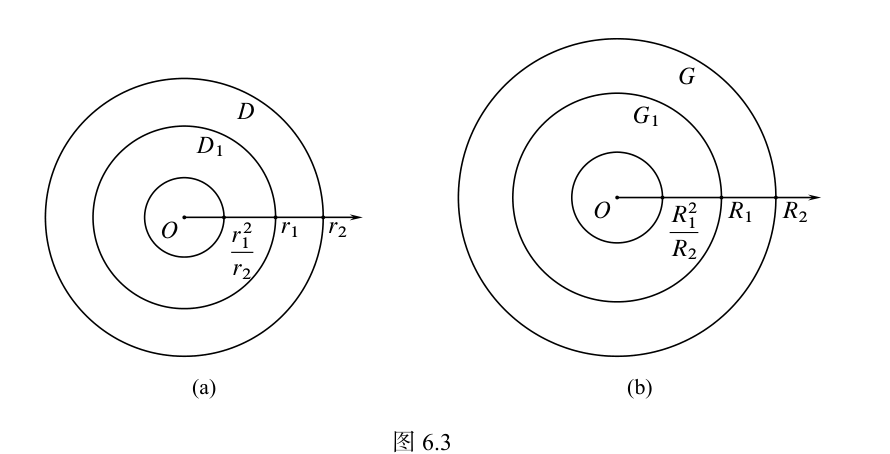
\includegraphics{public/figures/complex-functions/ch06-fig-6-3.png}

特别地，\(\operatorname{Aut}(A)=\{e^{i\theta}z,e^{i\theta}r_1r_2/z:\theta\in\mathbb R\}\)。量
\(\log(r_2/r_1)\) 称为圆环的模的一种归一化；若除以
\(2\pi\)，判别结论相同。

\Needspace{8\baselineskip}
\subsection{本节索引与方法}\label{ch06-s1-heading-7}

\hyperref[ch06-s1-heading-1]{Painlevé 原理} · \hyperref[ch06-s1-heading-2]{实轴反射} ·
\hyperref[ch06-s1-heading-3]{圆周反射} · \hyperref[ch06-s1-heading-4]{单叶条件修订} ·
\hyperref[ch06-s1-heading-5]{周期裂缝} · \hyperref[ch06-s1-heading-6]{圆环}

作反射题时，先明确源边界和目标边界，再写两次反射的复合，分别检查边界连续、分母不为零与两侧像的分离。全纯开拓存在与全局单叶是两项不同的结论。圆环题可以先看
\(\log|f|\) 的边值，再用闭路指标将连续参数压缩为整数。

\section{幂级数的全纯开拓}
对应教材第 201---206
页。一个幂级数不能在原收敛圆外直接求和，并不意味着其和函数不能开拓。换一个展开中心，新的收敛圆可能越过旧边界；真正的障碍是边界奇点。

\Needspace{8\baselineskip}
\subsection{定义 6.2.1：边界正则点与奇点}\label{ch06-s2-heading-1}

设 \(f\in H(D)\)、\(\zeta\in\partial D\)。若存在 \(\delta>0\) 及
\(g\in H(B(\zeta,\delta))\)，使 \(g=f\) 于整个
\(D\cap B(\zeta,\delta)\)，则称 \(\zeta\) 为 \(f\)
的正则点；否则称为奇点。这里的奇点是不能从原域跨过去的边界障碍；它不一定有完整的无心邻域，所以不一定属于第五章的孤立奇点分类。

正则点在 \(\partial D\)
中构成相对开集：一个开拓圆盘内更小的圆盘仍给出所需开拓。向函数加减一个在边界附近全纯的函数，不改变这里的正则性；特别地，修改幂级数的有限项不改变边界奇点。

设 \(f(z)=\sum_{n\ge0}a_nz^n\) 的收敛半径为
\(0<R<\infty\)，\(\zeta=Re^{i\theta}\)，取
\(z_0=te^{i\theta}\)，\(0<t<R\)。在 \(z_0\) 处重新展开：

\[
f(z)=\sum_{n=0}^{\infty}\frac{f^{(n)}(z_0)}{n!}(z-z_0)^n,
\qquad\rho\ge R-|z_0|.\qquad\text{(6.2.1)}
\]

若 \(\rho>R-|z_0|\)，新圆盘包含
\(\zeta\)，新旧和函数在两圆盘的交集上由唯一性定理一致，故能跨过
\(\zeta\)。反之，若 \(\zeta\) 正则，闭圆盘 \(\overline{B(z_0,R-|z_0|)}\)
除切点 \(\zeta\)
外全部位于原圆盘内；它因而包含在原圆盘与开拓邻域的并中。紧性给出一个稍大的同心圆盘仍在这个并中，故
Taylor 半径严格大于 \(R-|z_0|\)。所以对这样的径向内点，有

\[
\begin{aligned}
\zeta\text{ 正则}&\Longleftrightarrow\rho>R-|z_0|,\\
\zeta\text{ 奇异}&\Longleftrightarrow\rho=R-|z_0|.
\end{aligned}\qquad\text{(6.2.2)}
\]

\noindent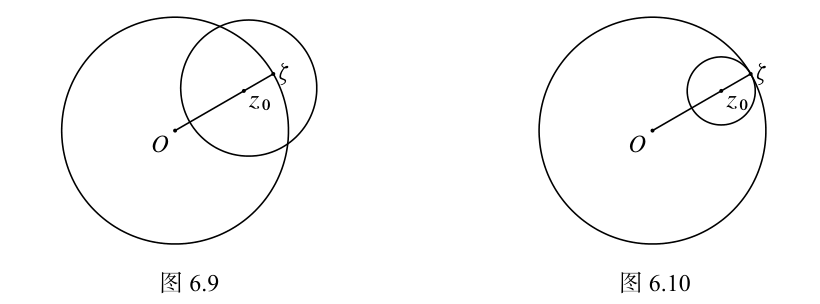
\includegraphics{public/figures/complex-functions/ch06-fig-6-9-10.png}

\Needspace{8\baselineskip}
\subsection{例 6.2.2：几何级数的唯一边界奇点}\label{ch06-s2-heading-2}

对 \(|z|<1\)，\(f(z)=\sum_{n\ge0}z^n=1/(1-z)\)。任取 \(|z_0|<1\)，

\[
\frac1{1-z}=\sum_{n=0}^{\infty}\frac{(z-z_0)^n}{(1-z_0)^{n+1}},
\qquad |z-z_0|<|1-z_0|.\qquad\text{(6.2.3)}
\]

系数的根值公式给出新半径恰为 \(|1-z_0|\)，它不小于 \(1-|z_0|\)，等号恰在
\(z_0\in[0,1)\) 成立。函数 \(1/(1-z)\) 在 \(\mathbb C\setminus\{1\}\)
全纯，而 \(z=1\) 是极点，因此单位圆上只有 \(1\) 是奇点。

原级数在单位圆上处处发散，因为通项不趋于零；但除 \(1\)
外的每一点都能跨越。这说明边界级数的收敛性与函数的可开拓性不能混同。

\Needspace{8\baselineskip}
\subsection{定理 6.2.3：收敛圆周上必有奇点}\label{ch06-s2-heading-3}

收敛半径满足 \(0<R<\infty\) 的幂级数，其和函数在 \(\partial B(0,R)\)
上至少有一个奇点。

证明：反设每个圆周点 \(\zeta\) 都正则，取开拓圆盘
\(B(\zeta,r_\zeta)\)。先核实这些局部函数能拼接。若两个圆盘相交，它们的交集连通，且交集必与
\(B(0,R)\) 相交：两个不同圆心间的开线段位于
\(B(0,R)\)，而两圆盘相交意味着可以在线段上选择一点同时满足到两圆心的距离小于对应半径；圆心相同则取其稍向内的点。交集因而有一块开集落在原圆盘内，两开拓函数在那里都等于
\(f\)，由唯一性定理在整个交集一致。

圆周紧，从中选出有限个圆盘覆盖圆周。把它们和 \(B(0,R)\) 合并成开集
\(U\)，上述一致性给出 \(F\in H(U)\)。\(U\) 包含紧集
\(\overline{B(0,R)}\)，所以存在 \(\varepsilon>0\)，使
\(B(0,R+\varepsilon)\subset U\)。\(F\) 在 \(0\) 处的 Taylor
系数仍为原来的 \(a_n\)，故原级数的收敛半径至少为
\(R+\varepsilon\)，矛盾。

有限正半径是必要前提：半径为无穷时没有有限收敛圆周；半径为零时连一个起始全纯函数元都没有。

\Needspace{8\baselineskip}
\subsection{命题 6.2.4：最终非负系数的正实奇点}\label{ch06-s2-heading-4}

若 \(\sum a_nz^n\) 的收敛半径为 \(0<R<\infty\)，且从某项起 \(a_n\)
都是非负实数，则 \(R\) 是其和函数的奇点。这是 Pringsheim
型结论；允许系数为零，尤其适用于缺项级数。

证明：减去有限多项的多项式，不改变收敛半径与边界奇点，可设所有
\(a_n\ge0\)。反设能在 \(B(R,\delta)\) 内开拓。取
\(0<h<\min(R/2,\delta/3)\)，令 \(x=R-h>0\)。圆盘 \(B(x,2h)\) 包含于
\(B(R,\delta)\)，所以开拓函数在 \(x\) 处的 Taylor
级数在该圆盘内收敛。由原圆盘内的逐项求导，

\[
b_k=\frac{f^{(k)}(x)}{k!}=\sum_{n=k}^{\infty}\binom nk a_nx^{n-k}\ge0.
\qquad\text{(6.2.4)}
\]

取 \(h<t<2h\)。Taylor 级数 \(\sum b_kt^k\)
有限，所有项非负，按非负级数换序与二项式公式得到

\[
\begin{aligned}
\sum_{k=0}^{\infty}b_kt^k
&=\sum_{n=0}^{\infty}a_n\sum_{k=0}^n\binom nk x^{n-k}t^k\\
&=\sum_{n=0}^{\infty}a_n(x+t)^n<\infty.
\end{aligned}\qquad\text{(6.2.5)}
\]

但 \(x+t>R\)，这与原收敛半径为 \(R\)
矛盾。非负性用来保证换序以及不存在抵消，不能把它换成``系数为实数''。

\Needspace{8\baselineskip}
\subsection{例 6.2.5：阶乘缺项与自然边界}\label{ch06-s2-heading-5}

设 \(f(z)=\sum_{n=0}^{\infty}z^{n!}\)。\(0!=1!=1\)
造成有限项重复，不影响结论。对 \(|z|<1\) 级数内闭一致收敛；在 \(z=1\)
发散，故收敛半径为 \(1\)。

取任意单位根 \(\eta=e^{2\pi ip/q}\)，\(q\ge1\)。当 \(n\ge q\) 时，\(q\)
整除 \(n!\)，所以

\[
f(\eta z)=\sum_{n<q}\eta^{n!}z^{n!}+\sum_{n\ge q}z^{n!}.
\qquad\text{(6.2.6)}
\]

减去前面的多项式后，系数全部非负，半径仍为 \(1\)。命题 6.2.4 表明
\(z=1\) 是 \(f(\eta z)\) 的奇点，即 \(\eta\) 是 \(f\)
的奇点。单位根在单位圆上稠密；若某圆周点正则，它的一个圆周邻弧全部正则，与稠密的奇点集矛盾。因此单位圆每点都是奇点，称为
\(f\) 的自然边界。

自然边界还意味着不存在包含原圆盘的严格更大域上的单值全纯开拓：若存在，连接圆内点与圆外点的域内路径必穿过某个圆周点，而该点附近就会给出不可能存在的局部开拓。

\Needspace{8\baselineskip}
\subsection{例 6.2.6：边界一致收敛仍然不能开拓}\label{ch06-s2-heading-6}

设

\[
g(z)=\sum_{n=1}^{\infty}\frac{z^{n!}}{n^2}.\qquad\text{(6.2.7)}
\]

在 \(|z|\le1\) 上，各项绝对值不超过
\(1/n^2\)，因此绝对一致收敛，和函数连续至闭圆盘。若
\(|z|>1\)，\(|z|^{n!}/n^2\) 不趋零，所以收敛半径仍为 \(1\)。对单位根
\(\eta\)，\(g(\eta z)\) 与最终非负系数的级数只差有限多项，仍由命题 6.2.4
得到 \(\eta\) 奇异，再由稠密性得到整个单位圆为自然边界。

与例 6.2.2 对照，可形成下面的准确比较：

\begin{longtable}[]{@{}lll@{}}
\toprule\noalign{}
幂级数 & 原圆周上的收敛 & 和函数跨圆周的能力 \\
\midrule\noalign{}
\endhead
\bottomrule\noalign{}
\endlastfoot
\(\sum z^n\) & 处处发散 & 除 \(1\) 外处处可开拓 \\
\(\sum z^{n!}\) & 每一点的通项模为 \(1\)，处处发散 & 单位圆是自然边界 \\
\(\sum z^{n!}/n^2\) & 绝对一致收敛 & 单位圆仍是自然边界 \\
\end{longtable}

\Needspace{8\baselineskip}
\subsection{本节索引与方法}\label{ch06-s2-heading-7}

\hyperref[ch06-s2-heading-1]{定义与换中心} · \hyperref[ch06-s2-heading-2]{几何级数} ·
\hyperref[ch06-s2-heading-3]{收敛圆周奇点} · \hyperref[ch06-s2-heading-4]{非负系数} ·
\hyperref[ch06-s2-heading-5]{阶乘缺项} · \hyperref[ch06-s2-heading-6]{一致收敛例}

判断可开拓性时，先寻找闭式或换中心后的半径；证明某点奇异时，可以利用极点、非负系数或已知奇点的变换。要证明自然边界，常用``先找稠密奇点，再利用正则点的相对开放性''。边界连续、绝对收敛和全纯跨越边界是三个不同层次。

\section{多值全纯函数与单值性定理}
对应教材第 206---209
页。先固定一个起始函数元，再沿路径逐段接续。局部唯一性保证同一路径的结果唯一；同伦不变性才把不同路径的结果联系起来。本节给出路径法证明，不预先调用第七章的
Riemann 映射或边界对应。

\Needspace{8\baselineskip}
\subsection{定义 6.3.1：函数元与沿路径的开拓}\label{ch06-s3-heading-1}

以 \(a\) 为中心、正收敛半径的幂级数 \(P(z)=\sum a_n(z-a)^n\)
称为一个函数元。讨论局部数据时，两个在 \(a\)
附近一致的全纯函数代表同一芽；其在 \(a\) 的 Taylor
系数相同。函数元可取自身最大收敛圆盘，也可暂时限制到较小圆盘作拼接，最终芽并不改变。

设 \(\gamma:[\alpha,\beta]\to\mathbb C\)
连续，\(\gamma(\alpha)=a\)。若有以 \(\gamma(t)\) 为中心的函数元
\(P_t\)，满足起始元为 \(P_\alpha=P\)，且对每个 \(t_0\)，所有充分接近
\(t_0\) 的 \(t\) 所对应圆盘相交、和函数在交集一致，就称 \(P\) 能沿
\(\gamma\) 全纯开拓，终点元是 \(P_\beta\)。

等价的局部表述更便于证明：每个 \(t_0\)
附近，可以用同一个全纯函数表示这些 \(P_t\) 在 \(\gamma(t)\)
的芽。由原定义到此表述，只须把时间邻域缩小到 \(\gamma(t)\) 落在
\(P_{t_0}\) 的一个较小圆盘内；反向由唯一性定理得到交叠一致。

沿路径开拓只使用连续性与局部全纯性，并不要求路径可微或可求长。只有把结果写成路径积分时，才另外要求相应的可求长条件。

\Needspace{8\baselineskip}
\subsection{例 6.3.2：径向开拓与边界奇点}\label{ch06-s3-heading-2}

设 \(P\) 的中心为 \(a\)、半径为 \(R>0\)。若 \(z_0\in B(a,R)\)，沿线段
\([a,z_0]\)，取和函数在每点的 Taylor 元便给出开拓。若
\(z_0\in\partial B(a,R)\)
是正则点，最后再接入一个跨边界的函数元，仍可沿闭线段开拓到终点。

反之，若 \(w_0\in\partial B(a,R)\) 是奇点，却能沿 \([a,w_0]\)
开拓，终点元会在 \(w_0\)
的某圆盘内全纯。靠近终点的内侧元与原和函数相同，终点元因而在与原圆盘的交集中一致，给出跨越
\(w_0\) 的开拓，矛盾。

教材本例中的圆心 \(B(0,R)\) 应按起始元中心统一为
\(B(a,R)\)；内点根本不属于定义 6.2.1
的边界奇点，故这里将内点和边界正则点分开表述。

\Needspace{8\baselineskip}
\subsection{例 6.3.3：对数绕一周的变化}\label{ch06-s3-heading-3}

在 \(z=1\) 取起始元

\[
P(z)=\sum_{n=1}^{\infty}\frac{(-1)^{n-1}}n(z-1)^n,
\quad |z-1|<1,\quad P(1)=0.\qquad\text{(6.3.1)}
\]

沿正向单位圆 \(\gamma(t)=e^{it}\)，\(0\le t\le2\pi\)，在每点取

\[
P_t(z)=it+\sum_{n=1}^{\infty}\frac{(-1)^{n-1}}n
\left(\frac{z-e^{it}}{e^{it}}\right)^n.
\qquad\text{(6.3.2)}
\]

该局部函数的导数为 \(1/z\)，在中心取值 \(it\)。对接近的
\(s,t\)，两局部函数之差导数为零；沿短圆弧积分 \(dz/z=i\,dt\)
又给出中心值的变化为
\(i(t-s)\)，所以两者在交集一致。这证明它们确实组成一族开拓，而不是仅凭多值符号猜测结果。

终点元为 \(P+2\pi i\)；负向绕一周则为 \(P-2\pi i\)。对以 \(1\)
为起终点的可求长闭路 \(\gamma\subset\mathbb C\setminus\{0\}\)，同理

\[
P_{\mathrm{end}}=P+\int_\gamma\frac{dz}{z}
=P+2\pi i\operatorname{Ind}(\gamma,0).\qquad\text{(6.3.3)}
\]

这说明起点、终点相同不能替代固定路径或端点固定的同伦。

\Needspace{8\baselineskip}
\subsection{命题 6.3.4：固定路径的唯一性}\label{ch06-s3-heading-4}

同一起始元沿同一条路径的开拓若存在，则在每个参数点的芽都唯一。

证明：设 \(P_t,Q_t\) 是两族开拓，令 \(E\) 为二者在 \(\gamma(t)\)
的芽相等的参数集合。固定 \(t_0\)，在 \(\gamma(t_0)\)
选一个公共小圆盘，分别以两个全纯函数 \(p,q\)
表示两族附近的芽；再缩小参数邻域，使附近中心都落在这个圆盘内。如果
\(p,q\)
在其中任何一个中心的芽相等，由唯一性定理它们在公共圆盘处处相等；如果不相等，则任一附近中心的芽也不相等。因此
\(E\) 和其补集都相对开。起始芽相同，所以 \(\alpha\in E\)；区间连通，得
\(E=[\alpha,\beta]\)。

两个直接推论也需要保留：将一族开拓的参数倒序，就得到反向路径的开拓，回到原来的起始元；在第一条路径的终点元处接上第二条路径的开拓，再重新参数化，就得到拼接路径的开拓。由唯一性，先接再反向的结果与这些操作一致。

\Needspace{8\baselineskip}
\subsection{定义 6.3.5：域上的多值全纯函数}\label{ch06-s3-heading-5}

固定 \(a\in D\) 处的函数元 \(P_0\)，要求它能沿 \(D\) 中从 \(a\)
出发的每一条路径开拓。对每个 \(z\in D\)，收集所有这些开拓到达 \(z\)
时的函数值，得到非空集合 \(f(z)\)，称为由 \(P_0\) 产生的多值全纯函数。

这里每一条路径是定义的一部分。某个代数表达式在多数点存在局部根，或一个函数导数处处非零，都不能自动保证其逆元能够沿像域中的任意路径一直开拓；可能遇到临界值，也可能因原像逃向定义域边界而中断。

若从 \(P_0\) 沿路径 \(\eta\) 到达芽 \(P\)，则 \(P\)
也能沿以该点为起点的任意路径开拓，因为可以先走 \(\eta\)
再走该路径。反过来先走 \(\eta^{-1}\) 回到
\(P_0\)，就能产生所有原来的芽。因此用任何一个可达芽作起点，都产生同一个多值函数。这也解释了为何定理
6.3.6 可以从指定的函数值出发。

\Needspace{8\baselineskip}
\subsection{同伦不变性的完整论证}\label{ch06-s3-heading-6}

\textbf{有限链与局部稳定引理。} 设起始元能沿 \(\gamma:[0,1]\to D\)
开拓。则存在 \(\varepsilon>0\)，使任何与 \(\gamma\) 一致距离小于
\(\varepsilon\)、起点和终点均相同的路径
\(\widetilde\gamma\)，都可沿同一有限函数链开拓，并得到相同的终点芽。

证明：由定义的局部表示与 \([0,1]\) 的紧性，选取分割
\(0=t_0<\cdots<t_N=1\) 和圆盘 \(U_j\Subset D\) 上的全纯函数 \(F_j\)，使
\(\gamma([t_{j-1},t_j])\) 紧含于 \(U_j\)。在每个接点 \(\gamma(t_j)\)
周围另取小圆盘 \(V_j\Subset U_j\cap U_{j+1}\)，使 \(F_j=F_{j+1}\) 于
\(V_j\)。这样的链可先从参数开覆盖取有限子覆盖，再取足够细的分割，每个闭子区间放在一个局部表示的参数邻域中。

各紧路径段到对应 \(\partial U_j\) 的距离均为正；各接点到
\(\partial V_j\) 的距离也为正。取 \(\varepsilon\)
小于这些有限个正数的最小值。于是 \(\widetilde\gamma\) 的每段仍在同一个
\(U_j\) 内，每个接点仍在相应 \(V_j\) 内，故 \(F_1,\ldots,F_N\)
给出相容的开拓。起点、终点固定，最初与最后的芽均未改变。

\textbf{同伦不变性。} 若起始元能沿 \(D\) 中以 \(a\)
为起点的所有路径开拓，而 \(\gamma_0,\gamma_1\) 在 \(D\)
内端点固定同伦，则二者给出相同终点芽。

证明：设 \(H:[0,1]^2\to D\) 是同伦，\(\gamma_s(t)=H(s,t)\)。每条
\(\gamma_s\) 都有开拓。固定 \(s_0\)，对 \(\gamma_{s_0}\)
使用局部稳定引理；由 \(H\) 在紧正方形上一致连续，当 \(s\) 接近 \(s_0\)
时，两路径一致距离足够小，终点芽相同。因此终点芽作为 \(s\)
的函数局部常值；参数区间连通，故始终不变。这里没有假定所有路径的 Taylor
半径事先有统一正下界，所需正余量来自每条固定路径的有限链。

\Needspace{8\baselineskip}
\subsection{定理 6.3.6：单值性定理}\label{ch06-s3-heading-7}

设 \(f\) 是域 \(D\)
上由函数元开拓产生的多值全纯函数，\(z_0\in D\)、\(w_0\in f(z_0)\)。若
\(G\subset D\) 单连通且 \(z_0\in G\)，则存在单值全纯分支
\(g\in H(G)\)，满足 \(g(z_0)=w_0\)，并且 \(g\) 在 \(z_0\) 的 Taylor
元经过 \(D\) 内的开拓仍产生整个 \(f\)。

证明：选一个到达 \(z_0\) 且取值为 \(w_0\) 的可达芽
\(P\)。反向与拼接性质保证 \(P\) 能沿 \(D\) 中每条路径开拓，且生成原来的
\(f\)。对 \(z\in G\)，任选 \(G\) 中从 \(z_0\) 到 \(z\)
的路径，以终点元在 \(z\) 的值定义
\(g(z)\)。单连通意味着任意两条这样的路径端点固定同伦，同伦不变性说明定义与路径无关，连终点芽也无关。

固定 \(z\)，取其终点芽的一个小圆盘 \(B(z,r)\subset G\)。到附近 \(w\)
的路径可先走到 \(z\) 再接一条圆盘内线段，故 \(g\)
在这整个小圆盘内等于同一个全纯函数。于是 \(g\in H(G)\)，起始值为
\(w_0\)，且起始 Taylor 元恰为
\(P\)。最后一个断言由换起始芽不改变可达芽族得出。

定理对 \(G=\mathbb C\) 同样由这段证明成立，不必先假定起始 Taylor
级数有无穷收敛半径。固定起始芽后分支唯一；仅固定一个函数值不一定确定芽。例如
\((\log z)^2\) 在 \(z=1\) 的两支 \((\operatorname{Log}z+2\pi i)^2\) 与
\((\operatorname{Log}z-2\pi i)^2\) 取值同为 \(-4\pi^2\)，导数却不同。

作为应用，若 \(q\in H(G)\) 在单连通域 \(G\) 内无零点，每点附近可对
\(q/q(z_0)\) 使用 \(\log(1+w)\)
的局部级数；沿紧路径取有限链，并调整相邻对数的 \(2\pi i\)
整数差，即可沿任意路径接续。定理便给出全纯对数 \(L\)；局部恒等式
\(e^L=q\) 由接续保持，因此 \(e^{L/m}\) 是全纯 \(m\)
次根。非单连通域则需检查闭路后芽是否回到原位，例如
\(\mathbb C\setminus\{0\}\) 上的 \(\log z\) 就不满足这一要求。

\Needspace{8\baselineskip}
\subsection{定理 6.3.7：Picard 小定理}\label{ch06-s3-heading-8}

若整函数 \(f\) 省略两个不同的有限值 \(a,b\)，则 \(f\) 为常函数。

\textbf{由已证导数估计得到的证明。} 令 \(F=(f-a)/(b-a)\)，则
\(F:\mathbb C\to\Omega=\mathbb C\setminus\{0,1\}\)。第五章 §5.2
的补充引理 A、B 已完整证明：存在 \(\Omega\) 上的正函数
\(\lambda\)，对任何全纯映射 \(H:B(0,R)\to\Omega\)，都有

\[
\lambda(H(z))|H'(z)|\le\frac{2R}{R^2-|z|^2}.
\qquad\text{(6.3.4)}
\]

该估计来自显式密度

\[
\lambda(w)=\frac{c(1+|w|^{1/4})(1+|w-1|^{1/4})}
{|w|^{7/8}|w-1|^{7/8}}
\]

及 \(\Delta\log\lambda\ge\lambda^2\) 的圆盘比较，不依赖 Riemann
映射、单值性或 Picard 小定理。固定
\(z_0\in\mathbb C\)，将式（6.3.4）用于任意半径圆盘 \(B(z_0,R)\)
的中心，得

\[
0\le\lambda(F(z_0))|F'(z_0)|\le\frac2R.
\]

令 \(R\to\infty\)，因 \(\lambda(F(z_0))>0\)，有 \(F'(z_0)=0\)。\(z_0\)
任意，所以 \(F\) 及 \(f\)
为常函数。完整的密度构造与比较证明见\href{/notes/c463439a440b0b9ea4b53175/\#定理-526picard-大定理}{第五章
§5.2 的 Picard 补证}；此处仅复用其中两个已证引理，不需要第五章紧性引理。

\textbf{从 Picard 大定理得到的另一证明。} 考察 \(h(\zeta)=f(1/\zeta)\)
在 \(0\) 的孤立奇点。若可去，\(f\)
在无穷远附近有界，加上紧圆盘内有界，Liouville 定理给出常值。若为 \(m\)
阶极点，存在 \(C\) 使大圆上 \(|f(z)|\le C|z|^m\)，Cauchy
系数估计令半径趋无穷，得到所有 \(m\) 阶以上 Taylor 系数为零，所以 \(f\)
是多项式；非常数多项式由代数基本定理取到每个有限值，不可能省略
\(a,b\)。若为本性奇点，已证的 Picard
大定理也禁止省略两个有限值。只剩常函数情形。

教材原证明通过第七章的 Riemann 映射、边界对应与习题 6.1.11
构造覆盖映射。这里只把上述两条依赖已闭合的路线作为本章证明；教材的几何路线保留到第七章讨论，不将未完成的覆盖构造写成已经验证。仅有一个满射的全纯函数，也不足以直接断言其逆元能沿任意路径开拓，还必须证明覆盖或等价的路径提升性质。

\Needspace{8\baselineskip}
\subsection{本章索引与作答流程}\label{ch06-s3-heading-9}

\hyperref[ch06-s3-heading-1]{函数元} · \hyperref[ch06-s3-heading-2]{径向开拓} ·
\hyperref[ch06-s3-heading-3]{对数绕行} · \hyperref[ch06-s3-heading-4]{固定路径唯一性} ·
\hyperref[ch06-s3-heading-5]{多值函数} · \hyperref[ch06-s3-heading-6]{同伦论证} ·
\hyperref[ch06-s3-heading-7]{单值性} · \hyperref[ch06-s3-heading-8]{Picard 小定理}

遇到开拓问题，先写清起始函数元及其取值，再指出可沿哪些路径接续；比较终点时，区分同一路径、端点固定同伦、仅端点相同。若要得到全域单值分支，必须同时验证任意路径可开拓与闭路无分支变化。使用逆函数时，导数非零只给局部逆，不自动保证全局路径提升。

\clearpage\section*{第六章习题}\phantomsection\addcontentsline{toc}{section}{第六章习题}
按教材印刷第 199---201、205---206、209 页收录，三节分别为 11、10、7
道，共 28
道主编号题。保留全部小问、教材提示和原题图，不附习题解答。\(B(a,r)\)
表示开圆盘，\(\overline{B(a,r)}\)
表示闭圆盘；涉及无穷远的闭包在扩充平面中理解。正文例题与定理证明另见三节讲义。

\hyperref[ch06-practice-heading-1]{习题 6.1} · \hyperref[ch06-practice-heading-2]{习题 6.2} ·
\hyperref[ch06-practice-heading-3]{习题 6.3}

\Needspace{8\baselineskip}
\subsection{习题 6.1}\label{ch06-practice-heading-1}

\par\Needspace{5\baselineskip}
\noindent\textbf{1.} 设域 \(D\) 关于 \(x\) 轴对称，\(f\) 在 \(D\)
上亚纯，\(f(D\cap\mathbb R)\subset\mathbb R\cup\{\infty\}\)。证明：若
\(z_0\in D\) 是 \(f\) 的极点，则 \(\bar z_0\) 也是 \(f\) 的极点，并且

\[
\operatorname{Res}(f,\bar z_0)=\overline{\operatorname{Res}(f,z_0)}.
\]

\par\Needspace{5\baselineskip}
\noindent\textbf{2.} 设域 \(D\) 关于圆周 \(\partial B(a,r)\) 对称，\(f\) 在 \(D\)
上亚纯，\(f(D\cap\partial B(a,r))\subset\partial B(A,R)\)。证明：若
\(z_0,w_0\in D\) 关于 \(\partial B(a,r)\) 对称，\(z_0\) 是 \(f(z)-A\)
的一阶零点，则 \(w_0\) 是 \(f\) 的一阶极点，并且

\[
\operatorname{Res}(f,w_0)=-\frac{R^2(w_0-a)^2}{r^2\overline{f'(z_0)}}.
\]

\par\Needspace{5\baselineskip}
\noindent\textbf{3.} 设 \(0<r<R<\infty\)，\(f\) 在
\(B(0,R)\setminus\overline{B(0,r)}\) 上全纯，在
\(B(0,R)\setminus B(0,r)\) 上连续。证明：若 \(f\) 在 \(\partial B(0,r)\)
上恒为零，则在 \(B(0,R)\setminus\overline{B(0,r)}\) 上也恒为零。

\par\Needspace{5\baselineskip}
\noindent\textbf{4.} 设 \(\gamma\) 是圆周 \(\partial B(a,R)\)
上的一段开圆弧。证明：若 \(f\) 在 \(B(a,R)\) 上全纯，在
\(B(a,R)\cup\gamma\) 上连续，并且在 \(\gamma\) 上恒为零，则 \(f\) 在
\(B(a,R)\) 上也恒为零。

\par\Needspace{5\baselineskip}
\noindent\textbf{5.} 将图 6.4 所示的单连通域 \(D\) 双全纯地映为上半平面。

\noindent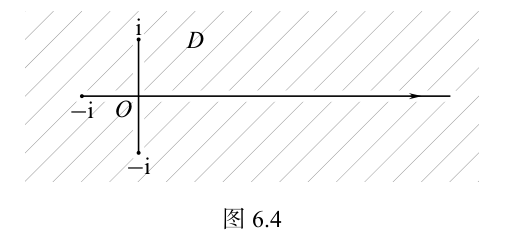
\includegraphics{public/figures/complex-functions/ch06-fig-6-4.png}

\par\Needspace{5\baselineskip}
\noindent\textbf{6.} 利用 Schwarz 对称原理证明：若 \(f\) 双全纯地将 \(B(a,r)\)
映为 \(B(A,R)\)，同胚地将 \(\overline{B(a,r)}\) 映为
\(\overline{B(A,R)}\)，则 \(f\) 必是分式线性变换。

\par\Needspace{5\baselineskip}
\noindent\textbf{7.} 设 \(P(x_1,x_2,\ldots,x_n)\) 是关于 \(x_1,x_2,\ldots,x_n\)
的多项式，\(f\in H(B(0,r))\)，\(\rho>1\)。证明：若在圆盘 \(B(0,r)\)
上成立

\[
f(z)=P\left(f\left(\frac z\rho\right),f'\left(\frac z\rho\right),
\ldots,f^{(n-1)}\left(\frac z\rho\right)\right),
\]

则 \(f\) 必能全纯开拓到 \(\mathbb C\)。

\par\Needspace{5\baselineskip}
\noindent\textbf{8.} 将图 6.5 所示的单连通域

\[
D=(\mathbb C\setminus[2,\infty))\setminus
\left(\overline{B(1,1)}\cup\overline{B(-1,1)}\right)
\]

双全纯地映为上半平面。

\noindent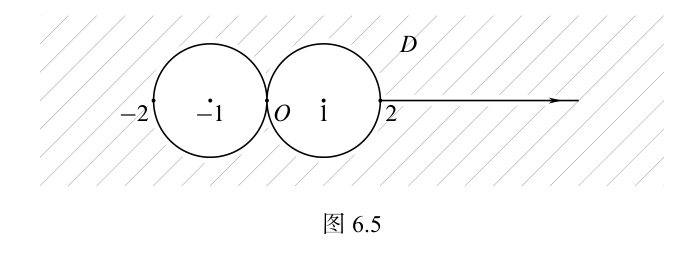
\includegraphics{public/figures/complex-functions/ch06-fig-6-5.png}

\par\Needspace{5\baselineskip}
\noindent\textbf{9.} 设 \(0<a<\infty\)，

\[
\begin{aligned}
L_k&=\{z=k\pi+\pi/2+iy:-a\le y\le a\},\quad k\in\mathbb Z,\\
D&=\left(\mathbb C\setminus\bigl(( -\infty,-\pi/2]\cup[\pi/2,\infty)\bigr)\right)
\setminus\bigcup_{k=-\infty}^{\infty}L_k.
\end{aligned}
\]

\(D\) 为图 6.6 所示的单连通域。将 \(D\) 双全纯地映为上半平面。

\noindent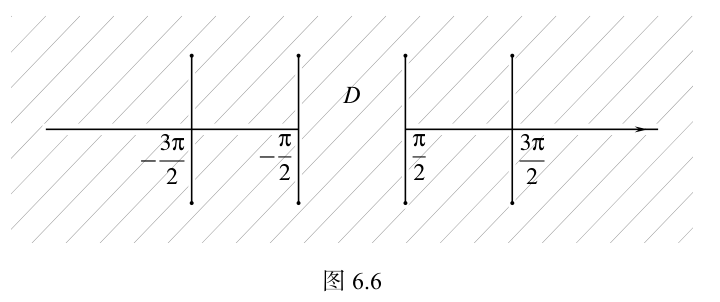
\includegraphics{public/figures/complex-functions/ch06-fig-6-6.png}

\par\Needspace{5\baselineskip}
\noindent\textbf{10.} 设
\(L_k=\{z=k\pi+iy:0\le y<\infty\}\)，\(k\in\mathbb Z\)，\(D=\mathbb C\setminus\bigcup_{k=-\infty}^{\infty}L_k\)
为图 6.7 所示的单连通域。将 \(D\) 双全纯地映为上半平面。

\noindent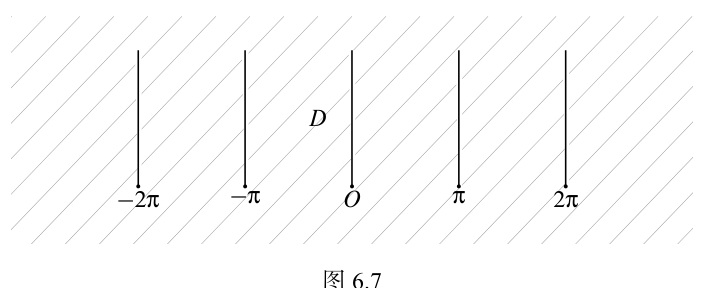
\includegraphics{public/figures/complex-functions/ch06-fig-6-7.png}

\par\Needspace{5\baselineskip}
\noindent\textbf{11.} 设 \(D\) 是由三条与 \(\partial B(0,1)\)
正交的圆弧所围成的单连通域，如图 6.8。证明：若 \(\varphi\) 双全纯地将
\(D\) 映为上半平面 \(\mathbb C^+=\{z:\operatorname{Im}z>0\}\)，同胚地将
\(\overline D\) 映为 \(\overline{\mathbb C^+}\)，\(A,B,C\) 分别映为
\(0,1,\infty\)，则 \(\varphi\) 可全纯开拓到 \(B(0,1)\)，且
\(\varphi(B(0,1))=\mathbb C\setminus\{0,1\}\)。

\noindent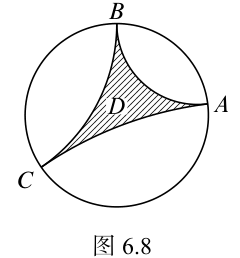
\includegraphics{public/figures/complex-functions/ch06-fig-6-8.png}

\subsubsection{本节校注}\label{ch06-practice-ux672cux8282ux6821ux6ce8}

第 2 题的残数公式按原书保留负号与导数上的共轭；所写有限点残数公式要求
\(z_0,w_0\in\mathbb C\)。若反射把圆心与无穷远交换，须另用局部坐标讨论，不能把
\(w_0=\infty\) 代入该式。第 8 题删去的是闭圆盘；第 9 题线段的下端为
\(-a\)。第 11 题的闭包包含球面上的无穷远点，圆弧端点位于单位圆上；本章
Picard 小定理已给出独立证明，不把本题的未解状态作为已完成的覆盖构造。

\Needspace{8\baselineskip}
\subsection{习题 6.2}\label{ch06-practice-heading-2}

\par\Needspace{5\baselineskip}
\noindent\textbf{1.}
证明：幂级数收敛圆周上的点是否为其和函数的奇点，与该幂级数的前有限项无关。

\par\Needspace{5\baselineskip}
\noindent\textbf{2.}
证明：若幂级数的收敛圆周上有其和函数的极点，则该幂级数在其收敛圆周上处处发散。

\par\Needspace{5\baselineskip}
\noindent\textbf{3.} 证明：若 \(\sum_{n=0}^{\infty}a_nz^n\)
的和函数在其收敛圆周上有一个一阶极点 \(z_0\)，此外再无其他奇点，则

\[
\lim_{n\to\infty}\frac{a_n}{a_{n+1}}=z_0.
\]

\par\Needspace{5\baselineskip}
\noindent\textbf{4.} 设 \(f(z)=\sum_{n=0}^{\infty}a_nz^n\) 的收敛半径为
\(1\)，\(F(w)=f(w/(1+w))=\sum_{n=0}^{\infty}b_nw^n\) 在原点的收敛半径为
\(\rho\)。证明：

(1) \(\rho\ge1/2\)，并且 \(-1\) 是 \(f\) 的奇点当且仅当 \(\rho=1/2\)；

(2) 若 \(1/2<\rho<1\)，则 \(f\) 能全纯开拓到
\(B(-\rho^2/(1-\rho^2),\rho^2/(1-\rho^2))\)；

(3) 若 \(\rho=1\)，则 \(f\) 能全纯开拓到
\(\{z:\operatorname{Re}z<1/2\}\)；

(4) 若 \(\rho>1\)，则 \(f\) 能全纯开拓到
\(\mathbb C\setminus\overline{B(\rho^2/(\rho^2-1),\rho/(\rho^2-1))}\)；

(5) 若 \(\rho=\infty\)，则 \(f\) 能全纯开拓到
\(\mathbb C\setminus\{1\}\)。

\par\Needspace{5\baselineskip}
\noindent\textbf{5.} 设 \(D\) 是域。证明：存在 \(f\in H(D)\)，使 \(\partial D\)
中的每个点皆是 \(f\) 的奇点。

\par\Needspace{5\baselineskip}
\noindent\textbf{6.} 证明：\(\sum_{n=0}^{\infty}z^{2^n}\)
的收敛圆周上的每个点皆为其和函数的奇点。

\par\Needspace{5\baselineskip}
\noindent\textbf{7.} 证明：\(\sum_{n=0}^{\infty}z^{2^n}/2^n\)
的收敛圆周上的每个点皆为其和函数的奇点。

\par\Needspace{5\baselineskip}
\noindent\textbf{8.} 设 \(f(z)=\sum_{n=0}^{\infty}a_nz^n\) 的收敛半径为
\(1\)，\(a_n\) 为实数，\(S_n=\sum_{k=0}^na_k\)。证明：若
\(S_n\to\infty\)，则 \(1\) 是 \(f\) 的奇点。举例说明，仅仅
\(|S_n|\to\infty\) 不能保证 \(1\) 是 \(f\) 的奇点。提示：考虑
\(f(z)/(1-z)\)。

\par\Needspace{5\baselineskip}
\noindent\textbf{9.} 证明：若 \(\sum_{n=0}^{\infty}a_nz^n\) 的收敛半径为
\(1\)，其和函数在 \(\partial B(0,1)\) 上有一阶极点
\(z_1,z_2,\ldots,z_m\)，此外再无其他奇点，则 \(\{a_n\}\) 有界。

\par\Needspace{5\baselineskip}
\noindent\textbf{10.} 若 \(f(z)=\sum_{n=0}^{\infty}a_nz^n\) 的收敛半径为
\(1\)，且 \(a_n\to0\)。证明：若 \(z_0\in\partial B(0,1)\) 不是 \(f\)
的奇点，则 \(\sum_{n=0}^{\infty}a_nz_0^n\) 收敛。

\subsubsection{本节校注}\label{ch06-practice-ux672cux8282ux6821ux6ce8-1}

第 4(2) 题按上传原书保留半径 \(\rho^2/(1-\rho^2)\)。由逆变换
\(w=z/(1-z)\) 直接解 \(|w|<\rho\)，实际得到更大的圆盘

\[
B\left(-\frac{\rho^2}{1-\rho^2},\frac\rho{1-\rho^2}\right).
\]

这是精确的逆像半径；原题给出的较小同心圆盘仍在其中，所以原题是较弱的结论，不能仅据半径不同就称其为错误命题。是否为排印失误尚未用另一版本核准。第
4
题各项中的``开拓到''均指与原圆盘的和函数相容后，在原域与所列区域的并上开拓；不能把不包含原圆盘的新圆盘直接叫作更大的原定义域。第
4(4) 题按有限 \(\rho>1\) 理解，无穷半径另列于 (5)。

\Needspace{8\baselineskip}
\subsection{习题 6.3}\label{ch06-practice-heading-3}

\par\Needspace{5\baselineskip}
\noindent\textbf{1.} 设 \(f\in H(D)\)，\(z_0\in D\)。证明

\[
F(z)=\int_{z_0}^zf(\zeta)\,d\zeta
\]

是 \(D\) 上的多值全纯函数。积分沿 \(D\) 中连接 \(z_0\) 和 \(z\)
的任意可求长曲线进行。

\par\Needspace{5\baselineskip}
\noindent\textbf{2.} 证明：若 \(f\) 是域 \(D\)
上非常数的全纯函数，但不是局部双全纯的，则 \(f^{-1}\) 一定不是域
\(G=f(D)\) 上的多值全纯函数。

\par\Needspace{5\baselineskip}
\noindent\textbf{3.} 举例说明，存在 \(B(0,1)\) 上的局部双全纯映射 \(f\)，使得
\(f^{-1}\) 不是域 \(G=f(B(0,1))\) 上的多值全纯函数。

\par\Needspace{5\baselineskip}
\noindent\textbf{4.} 证明：不存在 \(B(0,1)\) 上的局部双全纯映射 \(f\)，使
\(f(B(0,1))=\mathbb C\)，并且 \(f^{-1}\) 是 \(\mathbb C\)
上的多值全纯函数。

\par\Needspace{5\baselineskip}
\noindent\textbf{5.} 证明：不存在 \(B(0,1)\) 上的局部双全纯映射 \(f\)，使
\(f(B(0,1))=\mathbb C\setminus\{a\}\)，并且 \(f^{-1}\) 是
\(\mathbb C\setminus\{a\}\) 上的多值全纯函数。这里 \(a\in\mathbb C\)
为固定点。

\par\Needspace{5\baselineskip}
\noindent\textbf{6.} 求起始函数元

\[
f(z)=z^{1/2}=|z|^{1/2}e^{\frac i2\arg z}
=1+\sum_{k=1}^{\infty}\binom{1/2}{k}(z-1)^k
\]

沿单位圆周 \(\partial B(0,1)\) 正向与反向的全纯开拓；起点为
\(1\)，初始取值为 \(f(1)=1\)。

\par\Needspace{5\baselineskip}
\noindent\textbf{7.} 设幂级数族 \(\{P_t:\alpha\le t\le\beta\}\) 给出了沿平面曲线
\(z=\gamma(t)\) 的全纯开拓。证明：\(P_t\) 的收敛半径 \(R(t)\) 或者在
\([\alpha,\beta]\) 上恒为 \(\infty\)，或者是 \([\alpha,\beta]\)
上的正值连续函数。

\subsubsection{本节校注}\label{ch06-practice-ux672cux8282ux6821ux6ce8-2}

第 2---5 题的 \(f^{-1}\) 指包含全部原像的多值逆关系，是否满足定义 6.3.5
必须检查任意路径的全纯开拓。第 6 题把原书展开式隐含的起始分支 \(f(1)=1\)
明写出来，防止只写多值符号而漏掉函数元。第 7 题中的半径是每个完整 Taylor
级数的真实收敛半径，不能人为截小。


\end{document}
